\chapter{Gaussian Processes in 3D Face Registration}
The first of our two objectives is to build a face registration pipeline. In this context we use a stochastic process, more specifically a Vector-valued Gaussian process or Gaussian random field as the registration algorithm. In this chapter we explain the theory behind the implementation of the registration pipeline. To begin with, we recapitulate the definition
of stochastic processes and extend it to the definition of Gaussian processes. In the next step we introduce Gaussian Process Regression and finally explain how it can be applied 3D face mesh registration. 

\section{Stochastic Processes}
\begin{comment}
Assigns random variables to every point in time series or space 
\end{comment}

In probability theory a stochastic process consists of a collection of random variables $\{X(t)\}_{t \in \Omega}$ where $\Omega$ is an index set. It is used to model the change of a random value over time. The underlying parameter time is either real or integer valued (discrete). A generalization of a stochastic process, which is defined over space on an index set of d-dimensional vectors, is called a random field. 
\begin{comment}
A stochastic process is made up of a probability space (sample space, set of events, assignment of probabilities to events P: E → [0,1]) and a sigma-algebra (sample-space, €). It assigns a collection of random variables to an index set.
\end{comment}

\section{Gaussian Processes}

\begin{comment}
Definition taken from Stochastic Simulation p.306
\end{comment}

A Gaussian process is a stochastic process in which each finite collection $\Omega_{0} \subset \Omega$ of random variables has a joint normal distribution. More formally, we define each random variable in the collection of random variables $\{X(t)\}_{t \in \Omega}$ to have a d-dimensional normal distribution if the collection $\{X(t)\}_{t \in \Omega_{0}}$ - for any finite subset $\Omega_{0}$ - has a joint $d\times \left| \Omega_{0} \right|$-dimensional normal distribution with mean
$\mu (\Omega_{0})$ and covariance $\Sigma (\Omega_{0})$.  
If $\Omega \subseteq \mathbb{R}^{d}, d>1$ holds, the process is a Gaussian random field. In the further proceedings we will use the term ``Vector-valued Gaussian Processes'' to refer to Gaussian random fields. Defining the random variables on an index set in a d-dimensional space, allows for spatial correlation of the resulting values, which is an important aspect of the algorithm discussed later on.

\begin{comment} move to 3.4!! In our case, however, we use a collection of vector-valued random variables with indices in the $\mathbb{R}^{3}$ space because we want to model deformations of the vectors on the faces' surfaces.
\end{comment}
\begin{comment}
Now incorporate definition on p. 13 of Gaussian processes for machine learning
\end{comment}

\section{1-dimensional Gaussian Processes}
In order to familiarize the reader with Gaussian Processes, we start explaining the concept on the basis of an index set $\mathcal{X}$ of 1-dimensional inputs. To further simplify the concept it is possible to consider a Gaussian Process, or even any stochastic process, as a distribution over functions. Given a dataset, this circumstance allows us to look for inference in a space functions. Each random variable $X$ yields the value of a function $f(x)$ at a location $x \in
\mathcal{X}$ in the index set of possible inputs. The index set is denoted by $\mathcal{X}$ to stress that we are discussing Gaussian Processes defined over a space. In this function-space view a Gaussian Process at location $x$ is thus $f(x) \sim GP(\mu(x), k(x,x'))$ defined by its mean $\mu:\mathcal{X} \rightarrow \mathbb{R}$ and covariance $k:\mathcal{X} \times \mathcal{X} \rightarrow \mathbb{R}$ functions which in turn are defined over the set of inputs. With $\mu(\mathcal{X})=(\mu(x))_{x \in \mathcal{X}}$ and $\Sigma(\mathcal{X})=(k(x,x'))_{x,x' \in \mathcal{X}}$ we obtain the full distribution of the process $GP(\mu(\mathcal{X}),
\Sigma(\mathcal{X}))$. For the purpose of simplifying calculations we may assume that every random variable has zero mean without a loss of generality. (GP book)
\begin{comment}
Define Gaussian process for location x or for whole index set?
\end{comment}

\viscomment{define random variables as f or X now?}
\paragraph{Covariance Functions}
The key feature of a Gaussian Process is its covariance function also known as ``kernel''. It specifies the covariance $\mathbb{E}[f(x)f(x')]$ between pairs of random variables for two inputs $x$ and $x'$, allowing us to make assumptions about the input space by defining the spatial co-dependency of the modelled random variables. Note, that when assuming zero mean we can completely define the process' behaviour with the covariance function.\\
A simple example of a covariance function is the squared exponential covariance function, defined by $cov(f(x),f(x'))=k(x,x')=\exp(-\frac{(x-x')}{2l^{2}})$. (derivation Rasmussen et al. p.83) \begin{comment}
% future work: tweak parameters, try out other covariance functions
\end{comment}
It is possible to obtain different prior distributions by deploying different covariance functions. In our case, we use a stationary - meaning invariant to translation - isotropic, exponential covariance function - Squared Exponential Covariance Function (p. 38)

\begin{figure}[h!]
    \subfloat[Samples drawn from the prior]{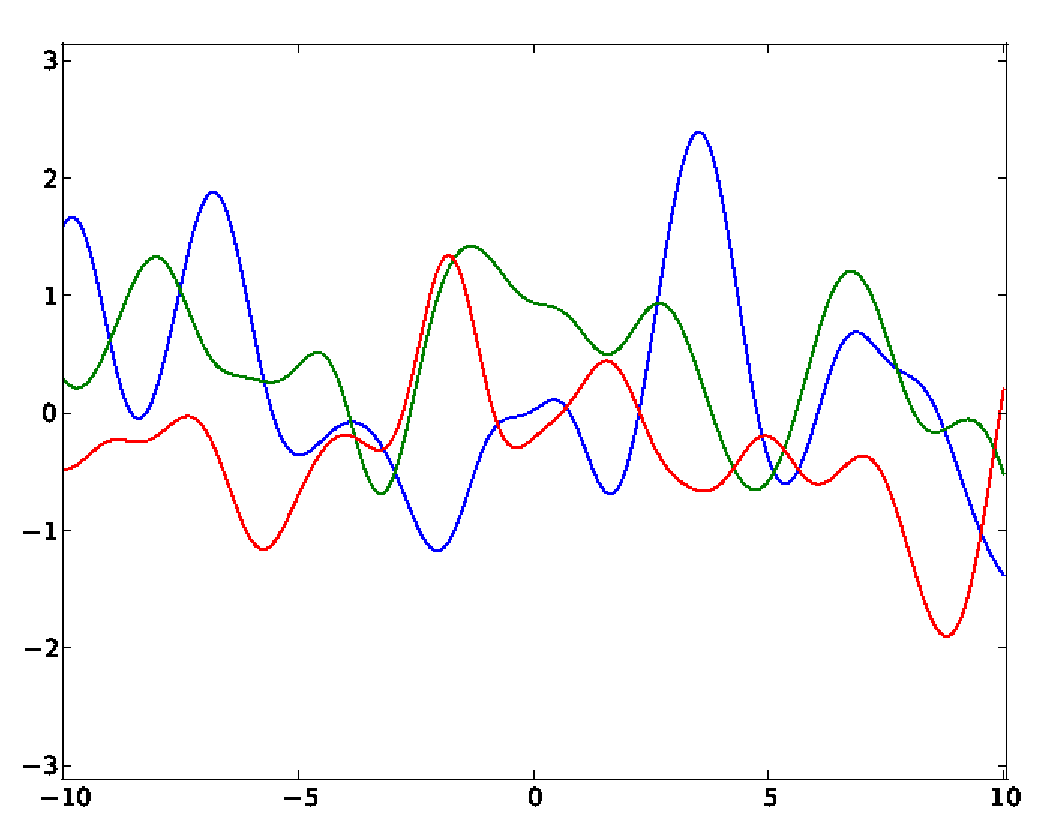
\includegraphics[width=.5\textwidth]{./resources/figures/gp_prior.eps}}
    \subfloat[Samples after a few observations]{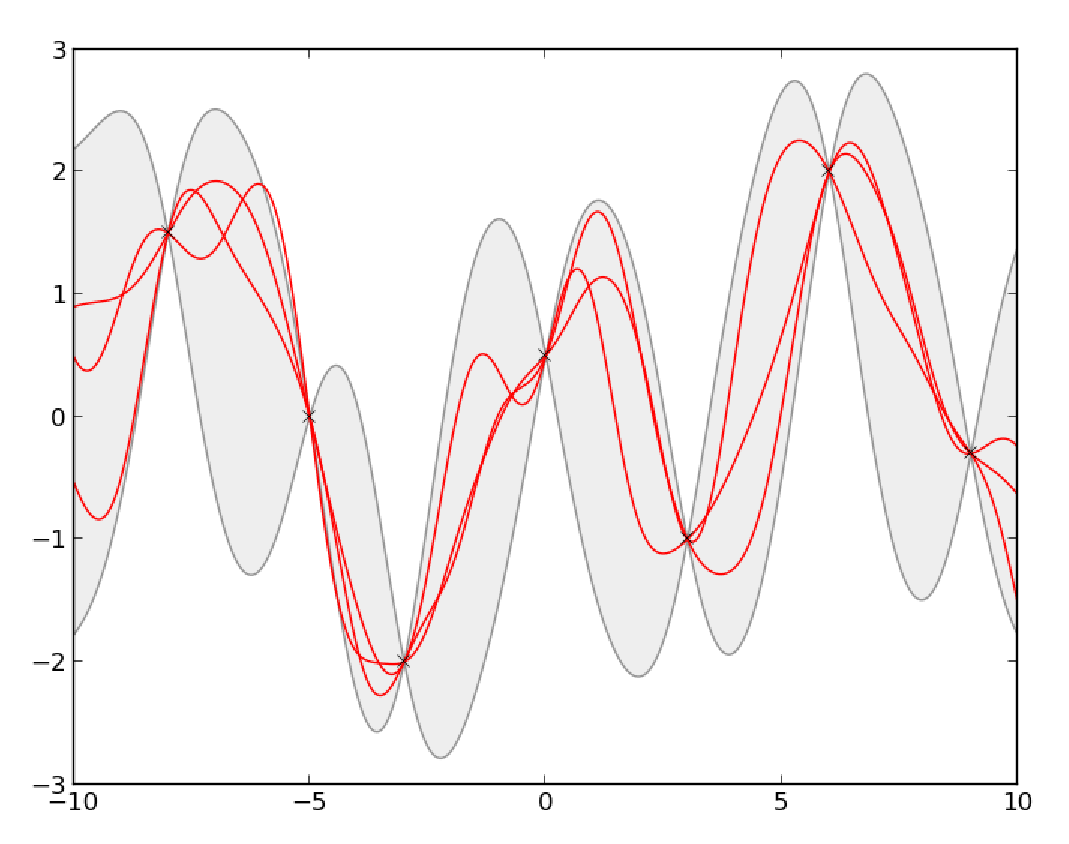
\includegraphics[width=.5\textwidth]{./resources/figures/gp_posterior.eps}}
\caption{In figure a) three functions have been drawn from the GP prior, each has a sample size of 1000 points. Figure b) again shows three functions, but this time the prediction incorporates the information of random values observed at seven points in the input space}
\label{fig:GPPlot}
% reference in text by \ref{$figure-name}
\end{figure}

\paragraph{Gaussian Process Prior}
The specification of the covariance function implies that a GP is a distribution over functions, because the covariance matrix is defined over function evaluations. To illustrate this one can draw samples from a prior distribution of functions evaluated at any number of points, $\mathcal{X}_{*}$. The Gaussian Process Prior is solely defined by the covariance matrix made up of the covariance function evaluations of the input points.

\begin{equation}
    \Sigma(\mathcal{X}_{*})=\begin{bmatrix}
k(x_{*1},x_{*2}) & \cdots & cov(f(x_{*1},f(x_{*n}) \\
\vdots & \ddots & \vdots \\
cov(f(x_{*n},f(x_{*1}) & \cdots & cov(f(x_{*n},f(x_{*n}) 
\end{bmatrix} \in \mathcal{M}^{\left|\mathcal{X}_{*}\right| \times \left|\mathcal{X}_{*}\right|} 
\end{equation}

A sample is a random Gaussian vector $\textbf{f}_{*} \sim \mathcal{N}(0, \Sigma(\mathcal{X}_{*}))$ containing a function value for every given input point. Plotting random
samples above their input points is a nice way of illustrating that a GP is indead a distribution over functions, see figure \ref{fig:GPPlot}. The GP Prior forms the basis for inference in Gaussian Process Regression.

\section{Gaussian Process Regression}
The task of registering a 3D template mesh with a scanned target mesh can be treated as a regression problem in which the goal is to predict the deformation field for all vertices in the template mesh, given the displacements of the template landmarks on to the target landmarks. Trying to fit an expected function - be it linear, quadratic, cubic or nonpolynomial - to the data is, however, not a sufficiently elaborated approach to our problem. 
Fortunately, using a Gaussian Process disposes of the need to describe the data by a specific function type, the response for every input point is instead represented by a normally distributed random variable, in turn governed by the specification of the covariance function. In short, we are modelling the space of possible regression functions through an infinite number of random variables in our input space. For the purpose of simplifying the concept of Gaussian Process Regression we will continue to stick with the examplory case of 1-dimensional inputs.

\paragraph{Regression Problem}
Assume a training set $\mathcal{S} = \{(x_{1},y_{1}), (x_{2},y_{2}), \cdots, (x_{n},y_{n})\}$ where $x \in \mathbb{R}$ and $y_{i}$ is a scalar output or target. 
\begin{comment}Later on, in the case of the training set consisting of landmarks, a Vector-valued Gaussian Process must be used, because y is then also a vector $y \in \mathbb{R}^{d}$.\end{comment} 
The task is now to infer the conditional distribution of the targets for yet unseen inputs $x_{*}$ given the training data $p(\textbf{f}_{*}\vert x_{*}, \mathcal{S})$

\paragraph{Noise-free Prediction}
First, we assume the observations from the training data to be noise-free so that we can fix the training data to these observations $\textbf{y}$ without complicating the model. The joint prior distribution with training $\textbf{f}$ and test $\textbf{f}_{*}$ outputs indicated is the following:

\begin{comment}
For every point we test, we extend the joint distribution by an input points, adding covariances and extending the dimensionality of the distribution
\end{comment}

\begin{equation}
\begin{bmatrix}\textbf{f}\\\textbf{f}_{*}\end{bmatrix}
\sim \mathcal{N}\left(\textbf{0},
\begin{bmatrix}
    \Sigma(X) & \Sigma(X,X_{*})\\
    \Sigma(X_{*},X) & \Sigma(X_{*})\\
\end{bmatrix}
\right)
\end{equation}

We obtain the posterior samples illustrated in \ref{fig:GPPlot} b) by conditioning the above joint Gaussian prior distribution on the observations $\textbf{f}_{*}\vert\textbf{f}=\textbf{y}$ which results in the following distribution:

\begin{comment}
reference equations for the conditional distributions
for example rasmussen: A.2 Gaussian Identities, p.200
\end{comment}

\begin{equation}
    \textbf{f}_{*}\vert X_{*},(X,\textbf{f}) \sim \mathcal{N}\left(\Sigma(X_{*},X)\Sigma(X)^{-1}\textbf{f},\\\Sigma(X_{*})-\Sigma(X_{*},X)\Sigma(X)^{-1}\Sigma(X,X_{*})\right)
\end{equation}

\begin{comment}Later on, we will extend this definition to 3-dimensional inputs and outputs.\end{comment}

\paragraph{Prediction with Gaussian Noise Model}
In most real world applications, however, observations from the training data are not free of noise. The landmarks clicked on the 3D face meshs, for example, can never be marked at the exact same feature location. These circumstances call for the incorporation of a noise model. We specify a simple additive i.i.d Gaussian noise model $y = f(x) + \varepsilon$ where $\varepsilon \sim \mathcal{N}(0, \sigma^2)$ for every input vector x. 

\begin{comment}In section \ref{} the variances will be varied for every sole landmark. For now it is enough to add the variance of the noise model to the covariance of the training.\end{comment}

\begin{equation}
\begin{bmatrix}\textbf{y}\\\textbf{y}_{*}\end{bmatrix}
\sim \mathcal{N}\left(\textbf{0},
\begin{bmatrix}
    \Sigma(X) + \sigma^2\mathcal{I}_{\left|X \right|} & \Sigma(X,X_{*})\\
    \Sigma(X_{*},X) & \Sigma(X_{*})\\
\end{bmatrix}
\right)
\end{equation}

The distribution - now conditioned on the noisy observations - is thus
\begin{subequations}
\begin{equation}
    \textbf{y}_{*}\vert \textbf{f}=\textbf{y} \sim \mathcal{N}\left(\overline{\textbf{y}}_{*} ,\Sigma(\textbf{y}_{*})\right)
\label{eq:3.5a}
\end{equation}
where the mean depends on the observed training targets 
\begin{equation}
    \overline{\textbf{y}}_{*} = \Sigma(X_{*},X)\left(\Sigma(X)+\sigma^2\mathcal{I}_{\left|X \right|}\right)^{-1}\textbf{y}
\end{equation}
whilst the covariance depends only on the input points
\begin{equation}
    \Sigma_{*} = \Sigma(X_{*}) - \Sigma(X_{*},X)\left(\Sigma(X)+\sigma^2\mathcal{I}_{\left|X \right|}\right)^{-1}\Sigma(X,X_{*})
\end{equation}
\end{subequations}
We have thus defined a Gaussian Process Posterior Model that contrains the 1-dimensional function space, fixed at the outputs of the training input points, between the training input points, as can be viewed in fig. \ref{fig:GPPlot} b). 
  
\section{Application to 3D Face Meshs} 
In this section of we adapt the above presented GP regression theory to our case of 3D face mesh registration. The task at hand is to register a reference or \textbb{template} face mesh with a scanned face mesh. We therefore strive to predict a deformation field $\mathcal{D}:\mathcal{M} \subset \mathbb{R}^3 \rightarrow \mathbb{R}^3$ which assigns a displacement vector to every vertex in the template mesh. During registration we refer to the template as the moving mesh
$\mathcal{M}$. Adding the deformation field to the moving mesh should then provide an accurate mapping to the target mesh $\mathcal{T}$ and thereby perform the registration. Our objective is to register the template with the set of scanned faces. 

Von skalarwertiger Funktion zu vektorwertiger Funktion, siehe Block!
\paragraph{Vector-valued Gaussian Processes}
In order to use Gaussian Processes to model deformation fields of three dimensional vectors as intended, there is the need for a generalization of the definition from the function-space view. The random variables $X_{1}, X_{2}, \ldots, X_{k}, \ldots, X_{n}$ are now d-dimensional vectors, yielding a vector-valued covariance function of the form $k: \mathcal{X} \times \mathcal{X} \rightarrow \mathbb{R}^{d \times d}$ and $k(x,x')=\mathbb{E}[X_{k}(x)^{T}X_{k}(x')]$ and mean function $\mu:
\mathcal{X} \rightarrow \mathbb{R}^{d}$. 

\paragraph{Reference Mesh Prior}
As defined by the deformation field the output the regression problem is in $\mathbb{R}^3$ calling for the use of a Vector-valued Gaussian Process with random variables $\delta \subseteq \mathbb{R}^3$ where $\delta$ stands for deformation. 
After the template and target have been aligned \ref{chapter 4} a Vector-valued Gaussian Process can be initialized by constructing a GP Prior of smooth deformations over all $n$ vertices of the template mesh. For this purpose the covariance function has to be redefined to handle 3-dimensional vectors.
\begin{equation}
    k\left(
    \begin{bmatrix}x_{1}\\x_{2}\\x_{3}\end{bmatrix},
    \begin{bmatrix}x'_{2}\\x'_{2}\\x'_{3}\end{bmatrix}
    \right) = x y^T \in M^{3 \times 3}
\end{equation}
Each covariance entails 9 relationships between the different components of the vectors, yielding a $3 \times 3$ matrix. The covariance matrix then grows to become: 
\begin{equation}
    \Sigma_{\mathcal{X}} = 
\begin{bmatrix}
    k(\vect{x}_{1},\vect{x}_{1}) & \cdots & k(\vect{x}_{1},\vect{x}_{n}) \\
\vdots & \ddots & \vdots \\
k(\vect{x}_{n},\vect{x}_{1}) & \cdots & k(\vect{x}_{n},\vect{x}_{n})
\end{bmatrix} \in M^{3n \times 3n}
\end{equation}

The template mesh is defined by a finite set of vectors $\mathcal{X} \in \mathbb{R}^3$ and a set of landmarks $L_\mathcal{M}=\{l_{\mathcal{M}1}, \cdots, l_{\mathcal{M}n}\} \subset \mathbb{R}^3$.
The mean vector $\mu$ is made up of the component-wise listing of vectors so that it has dimensionality $3n$. Setting the whole mean vector to zero, as discussed before, implies a mean deformation of zero and makes perfect sense in this setting, because we are modelling deformations of the template surface. 
The prior distribution over the template mesh is therefore defined as 
\begin{equation}
    \mathcal{D} \sim \mathcal{N}(\vect{0}, \Sigma_{\mathcal{X}})
\end{equation}
meaning that a sample deformation field can be directly drawn from the prior distribution of the template mesh.
\begin{figure}[h!]
    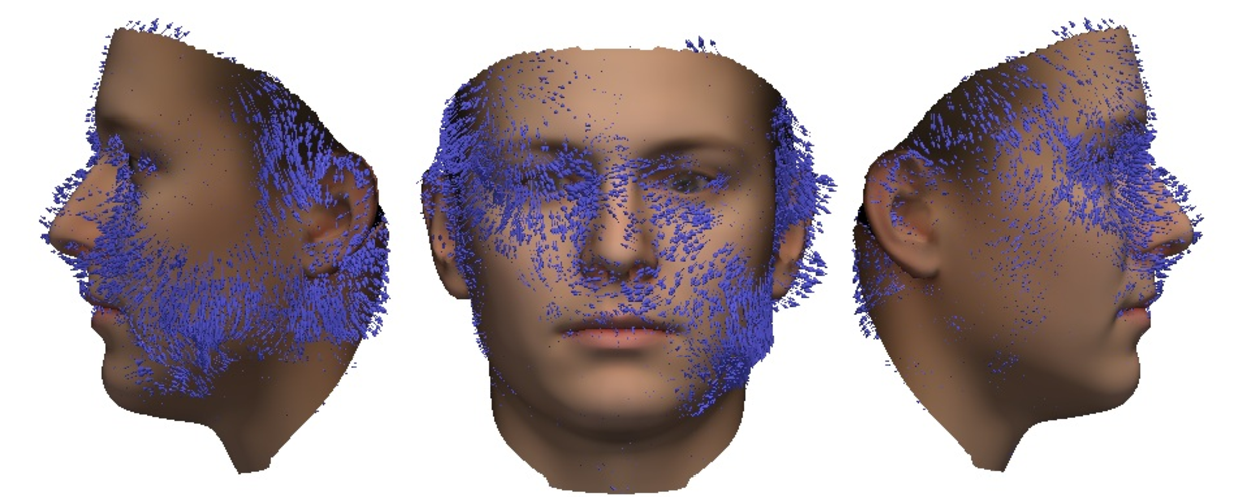
\includegraphics[width=\textwidth]{./resources/img/prior_deformations.pdf}
    \caption{A sample \textbf{prior} deformation field - depicted with a set of \textcolor{blue}{blue arrows} on the textured template face.}
\label{fig:priordeformations}
% reference in text by \ref{$figure-name}
\end{figure}
\paragraph{Reference Mesh Posterior}
The target landmarks also consist of a set $L_{\mathcal{T}} = \{l_{\mathcal{T}1},\cdots, l_{\mathcal{T}n}\} \subset \mathbb{R}^3$. 
Fixing the prior output to the deformation vectors $\mathcal{Y}=\{\vect{t}-\vect{m}\vert \vect{t} \in L_{\mathcal{T}}, \vect{m} \in L_{\mathcal{M}}\}$ - defined by the difference vectors between the template and target landmarks - and assuming additive i.i.d Gaussian noise, the resulting posterior distribution is
\begin{equation}
    \begin{bmatrix}\mathcal{Y_{\varepsilon}}\\\mathcal{D}\end{bmatrix}
\sim \mathcal{N}\left(\textbf{0},
\begin{bmatrix}
    \Sigma(\mathcal{Y}) + \sigma^2\mathcal{I}_{3\left|\mathcal{Y} \right|} & \Sigma(\mathcal{Y},X_{*})\\
    \Sigma(X_{*},\mathcal{Y}) & \Sigma(X_{*})\\
\end{bmatrix}
\right)
\end{equation}

The deformation model is now rendered approximately fixed at the landmarks in the target mesh and the goal is to find valid deformations through this set of fixed targets, analogous to the case of eq. \ref{eq:3.5a}. In other words the known respective displacements at the template landmarks co-define the distribution of possible deformations of all vertices in the template mesh.
\begin{figure}[h!]
    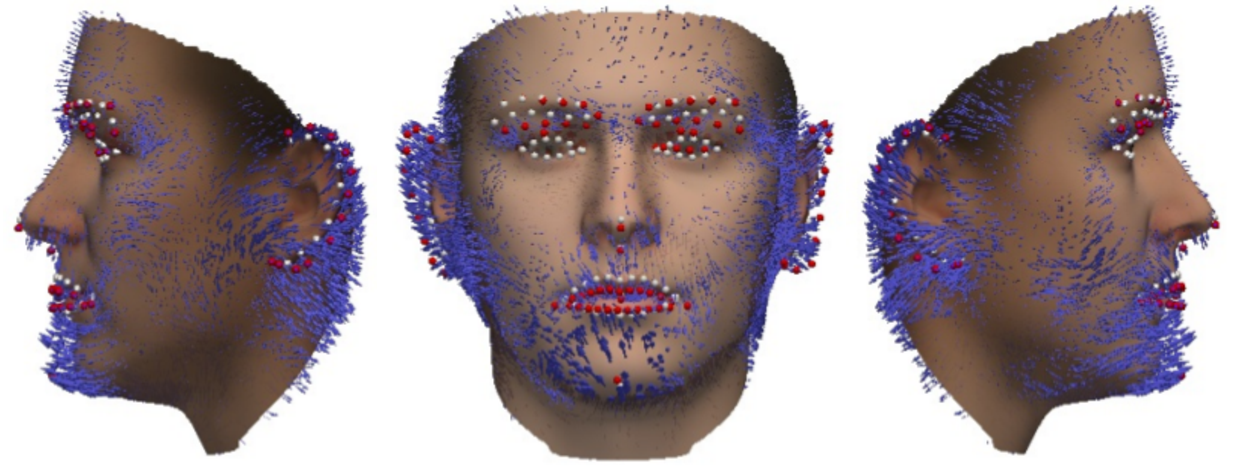
\includegraphics[width=\textwidth]{./resources/img/posterior_deformations.pdf}
    \caption{a sample \textbf{posterior} deformation field depicted with a set of \textcolor{blue}{blue arrows} on the textured template face. The white spheres are the landmarks of the template mesh which are mapped on to the \textcolor{red}{red landmarks} of the target.}
\label{fig:posteriordeformations}
\viscomment{make same images without line features and display instead}
\end{figure}
The posterior model is defined as the joint distribution of all template mesh points and the
template landmarks, conditioned on the respective displacement vectors for every template landmark with added noise. 
\begin{center}
\begin{equation}
    \mathcal{D}\vert \mathcal{X} \rightarrow \mathcal{Y}_{\varepsilon}. 
\end{equation}
\end{center}
\begin{figure}[h!]
    \centering
    \subfloat[Posterior mesh with target landmarks]{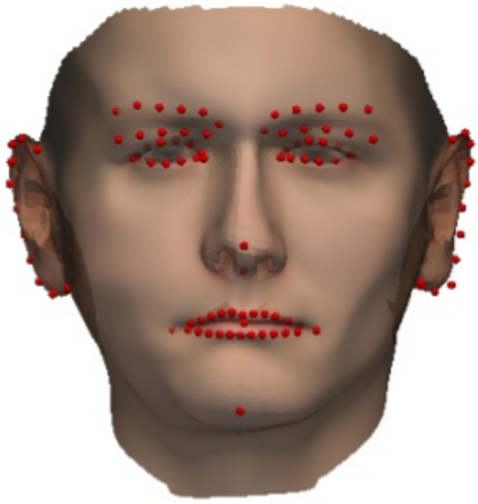
\includegraphics[width=.4\textwidth]{./resources/img/posterior_deformation_landmarks_front.pdf}}
    \quad\quad
    \subfloat[Prior mesh]{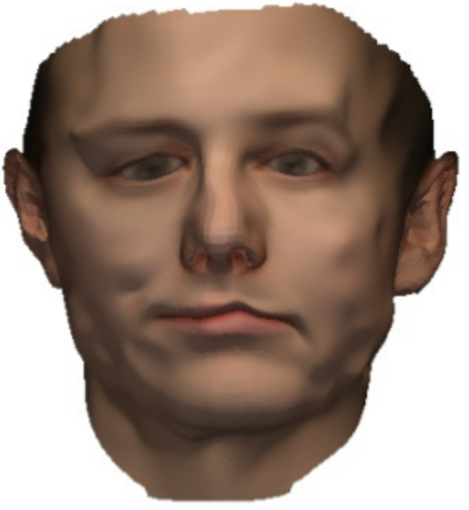
\includegraphics[width=.4\textwidth]{./resources/img/deformation_prior_msh.pdf}}
    \caption{a) is a posterior mesh, obtained by adding a sample deformation field to the template. In comparison to the mesh in b) the mesh in a) is much more face-like. The reason for this that the displacement of the landmarks has constricted the space of deformations to solely admissible deformations}
\label{fig:meshposterior}
\end{figure}
We now have defined a distribution over our template mesh. Sampling the conditional distribution and adding the resulting deformation onto the template creates deformed 3D surfaces of the template mesh which are fixed at the target landmarks \ref{fig:meshposterior}.

\section{Fitting \& Optimization}
\label{optimization}
In the previous paragraph we modelled the space of feasible deformations as a vector-valued Gaussian Process. Due to the fact that the posterior model is fixed at the target landmarks it is possible to perform the registration by drawing a shape from the posterior model. The sample, however, has to be optimized according to the shape of the target face. 
In order to find the deformation corresponding to the optimal fit $d_{*}$ a linear optimization is employed. \begin{equation}
    d_{*} = \underset{d \in \mathbb{D}}{\textbf{arg min}}\quad L[\mathcal{T}, \mathcal{M }\circ d]+\lambda R[d]
\end{equation}
Therein the deformation vectors of the landmarks and the posterior process act as constraints in the regularization term R. Minimizing the loss function L - for example the mean square error (MSE) - on the target and the deformed template should provide us with the optimal deformation under the given constraints. $\mathbb{D}$ denotes the space of possible deformations in the posterior model.\\ 

The problem with the above approach to optimization is that the deformations are modelled by a distribution and are therefore non-parametric. In order to properly perform optimization, however, we need a representation that can be controlled through/ is governed by a set of parameters. For this purpose we would like to specify a parametric model $\mathbb{M}[\alpha](x)=\mu(x)+ \sum^{n}_{i=1} \alpha_{i}\lambda_{i}\phi_{i}(x)$ which is defined over a finite set of basis
functions. The question remains how the Gaussian Posterior Model can be expressed as a linear model. Fortunately, the answer lies in Mercer's Theorem. It states that a symmetric, non-negative definite, continuous function $k$ can be expressed by the following linear combination of a countable sequence of functions $\{\phi_{i}\}_{i \in \mathbb{N}}$
\begin{equation}
    k(x,x') = \sum^{\infty}_{i=1}\lambda_{i}\phi_{i}(x)\phi_{i}(x') \in \mathbb{R}^{3 \times 3}
\end{equation}
Through the theorem we can define the covariance function of the our Gaussian Process Posterior in an infinite dimensional space made up of its eigenvalues $\lambda_{i}$ and eigenvectors $\phi_{i}: \mathbb{R}^3 \rightarrow \mathbb{R}^3$ which are functions in this case.
This infinite basis of functions corresponds to all possible deformations at a specific vertex in the template mesh. By evaluating a basis function at every vertex we receive a basis deformation field. We can further use Mercer's theorem to obtain the sought parametric model by estimating the covariance function. In order to achieve this a low-rank approximation of the covariance function - in terms of the first leading terms of its Mercer expansion - is performed $k(x,x') =
\sum^{n}_{i=1}\lambda_{i}\phi_{i}(x)\phi_{i}(x')$. For this to work the modelled deformations have to be sufficiently smooth, because we are disregarding a number of basis functions. Smoothness is guaranteed by the square exponential covariance function.
We can further express the deformation at a given mesh vertex by a linear combination of the selected basis functions and their eigenvalues with $\alpha_{1} \cdots \alpha_{n} \in \mathbb{R}$ as the linear parameters
\begin{equation}
f(x) = \sum^{n}_{i=1} \alpha_{i}\lambda_{i}\phi_{i}(x)
\end{equation}
In effect, we have formulated the Gaussian Process Registration problem in parametric form. Next, we want to minimize the residuals for all the points on the template surface according to optimal parameter values $\alpha_{i}$ 
\begin{equation}
    \underset{\alpha \in \mathbb{R}^n}{\textbf{arg min}}\quad \Sigma_{x_{i} \in \mathcal{M}} (f(x_{i}) - \varphi_{T}(x_{i}))^2
\end{equation}
where $f(x_{i})$ is the deformation function and $\varphi_{T}(x_{i})$ returns the nearest point on the target mesh. The optimization problem therefore becomes
\begin{equation}
    \alpha_{*} = \underset{\alpha \in \mathbb{R}^n}{\textbf{arg min}}\quad L[\mathcal{T}, \mathcal{M }\circ \mathbb{M}[\alpha]]+\lambda R[\alpha]
\end{equation}

Write as statistical PCA based shape model

\begin{comment}
Yields the overall loss function $\Phi_{L}$ 
\begin{equation}
\Phi_{L}(f(x_{i})-\varphi_{T}(x_{i}))
\end{equation}
Mercer's theorem analogue to eigenvalue decomposition
An alternative way of viewing the process is the eigenvalue decomposition of the whole covariance matrix
The information needed is held by the covariance matrix of the posterior process. 
K = sum over lambda times eigenvectors
http://www.quora.com/Mathematics/Can-you-explain-Mercers-Theorem
They denote the deformation directions while the eigenvalues \ldots
ne eigenvalue function by itself returns a global basis deformation when applied to every vertex. 
The eigen vectors - which are deformation vectors defining a deformation for every model vertex - of the covariance matrix define a basis space? 
Shape Modell => select best eigenvectors via PCA in order to simplify computation.
=> Vorstellen wie wenn mehrere Wellbleche durch die Target"\_"landmarks gelegt werden und dann mit bestimmten parametern alpha zwischen ihnen interpoliert wird
Alternative way to understand basis functions for gaussian process:
sample from the GP(0, K)
and then build a linear model from the functions, f(x) = sum(i, n) alpha(i) si(x)
Posterior Distribution of Landmarks
Defining the Gaussian Process
Posterior Distribution - Landmarks (Referenz deformieren 
From Gaussian Processes to Shape Models => by selected principal components of the covariance matrix
\end{comment}

